GPU是一种并行计算平台,它可以加速计算机的计算任务。CUDA是一种基于GPU的编程语言,它可以用来编写高性能的并行程序。

\subsection{CUDA简介}

2006年,NVIDIA公司发布了\textbf{CUDA}(Compute Unified Device Architecture),是一种新的操作\textbf{GPU}计算的硬件和软件架构,
是建立在NVIDIA的GPUs上的一个通用并行计算平台和编程模型,它提供了GPU编程的简易接口,基于CUDA编程可以构建基于GPU计算的应用程序,利用GPUs的\textbf{并行计算}引擎来更加高效地解决比较复杂的计算难题。
它将GPU视作一个数据并行计算设备,而且无需把这些计算映射到图形API。
操作系统的多任务机制可以同时管理CUDA访问GPU和图形程序的运行库,其计算特性支持利用CUDA直观地编写GPU核心程序。

CUDA提供了对其它编程语言的支持,如C/C++,Python,Fortran等语言。
只有安装CUDA才能够进行复杂的并行计算。主流的深度学习框架也都是基于CUDA进行GPU并行加速的,几乎无一例外。
还有一个叫做$cudnn$,是针对7\textbf{深度卷积神经网络}的加速库。

CUDA在软件方面组成有:一个CUDA库、一个应用程序编程接口(API)及其运行库(Runtime)、
两个较高级别的通用数学库,即CUFFT和CUBLAS。CUDA改进了DRAM的读写灵活性,
使得GPU与CPU的机制相吻合。另一方面,CUDA提供了片上(on-chip)共享内存,
使得线程之间可以共享数据。应用程序可以利用共享内存来减少DRAM的数据传送,
更少的依赖DRAM的内存带宽。

\subsection{配置CUDA环境}

CUDA编程语言是一种高级语言,需要安装CUDA编程环境才能进行编程。

\subsubsection{安装CUDA toolkit}

CUDA toolkit包括CUDA运行库、CUDA编程接口等内容,使我们使用CUDA加速程序开发的
基础。CUDA toolkit可以从NVIDIA官网下载,也可以从CUDA官方网站下载。

我们下面示例如何在\textbf{Ubuntu22.04}上安装\textbf{CUDA11.8}。需要注意的是,
CUDA与Ubuntu和GPU的版本有关,不同版本的Ubuntu可能需要不同的CUDA版本。
大家在安装时需要务必注意。

\begin{tbash}
# 下载CUDA安装包(这是一句长长的命令)
wget 
https://developer.download.nvidia.com/compute/cuda/11.8.0
/local_installers/cuda_11.8.0_520.61.05_linux.run

# 运行安装包
sudo sh cuda_11.8.0_520.61.05_linux.run
\end{tbash}

然后稍等片刻就可以看到这个界面

\begin{figure}[H]
    \centering
    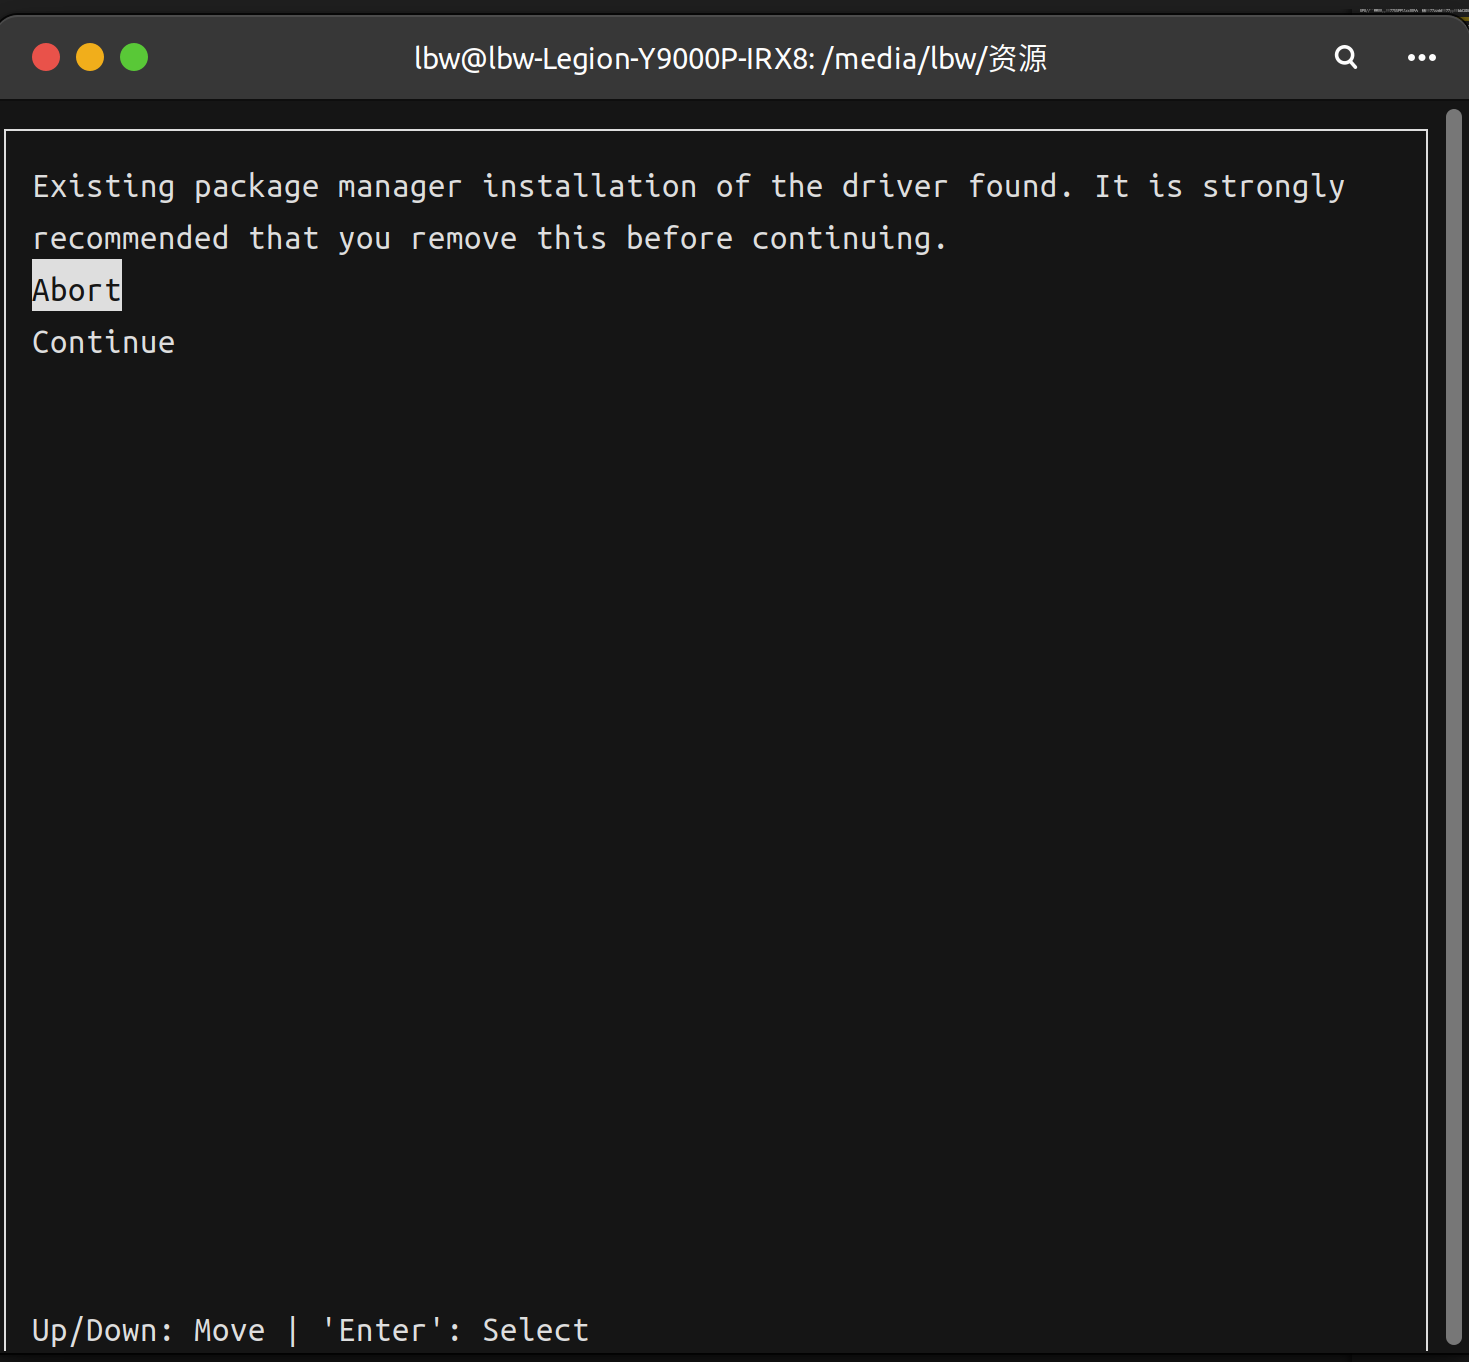
\includegraphics[width=0.7\textwidth]{CUDA_install.png}
    \caption{Step1} % 图片标题
    \label{fig:CUDA_install} % 图片标签,用于引用
\end{figure}

选择\textbf{Continue},

\begin{figure}[H]
    \centering
    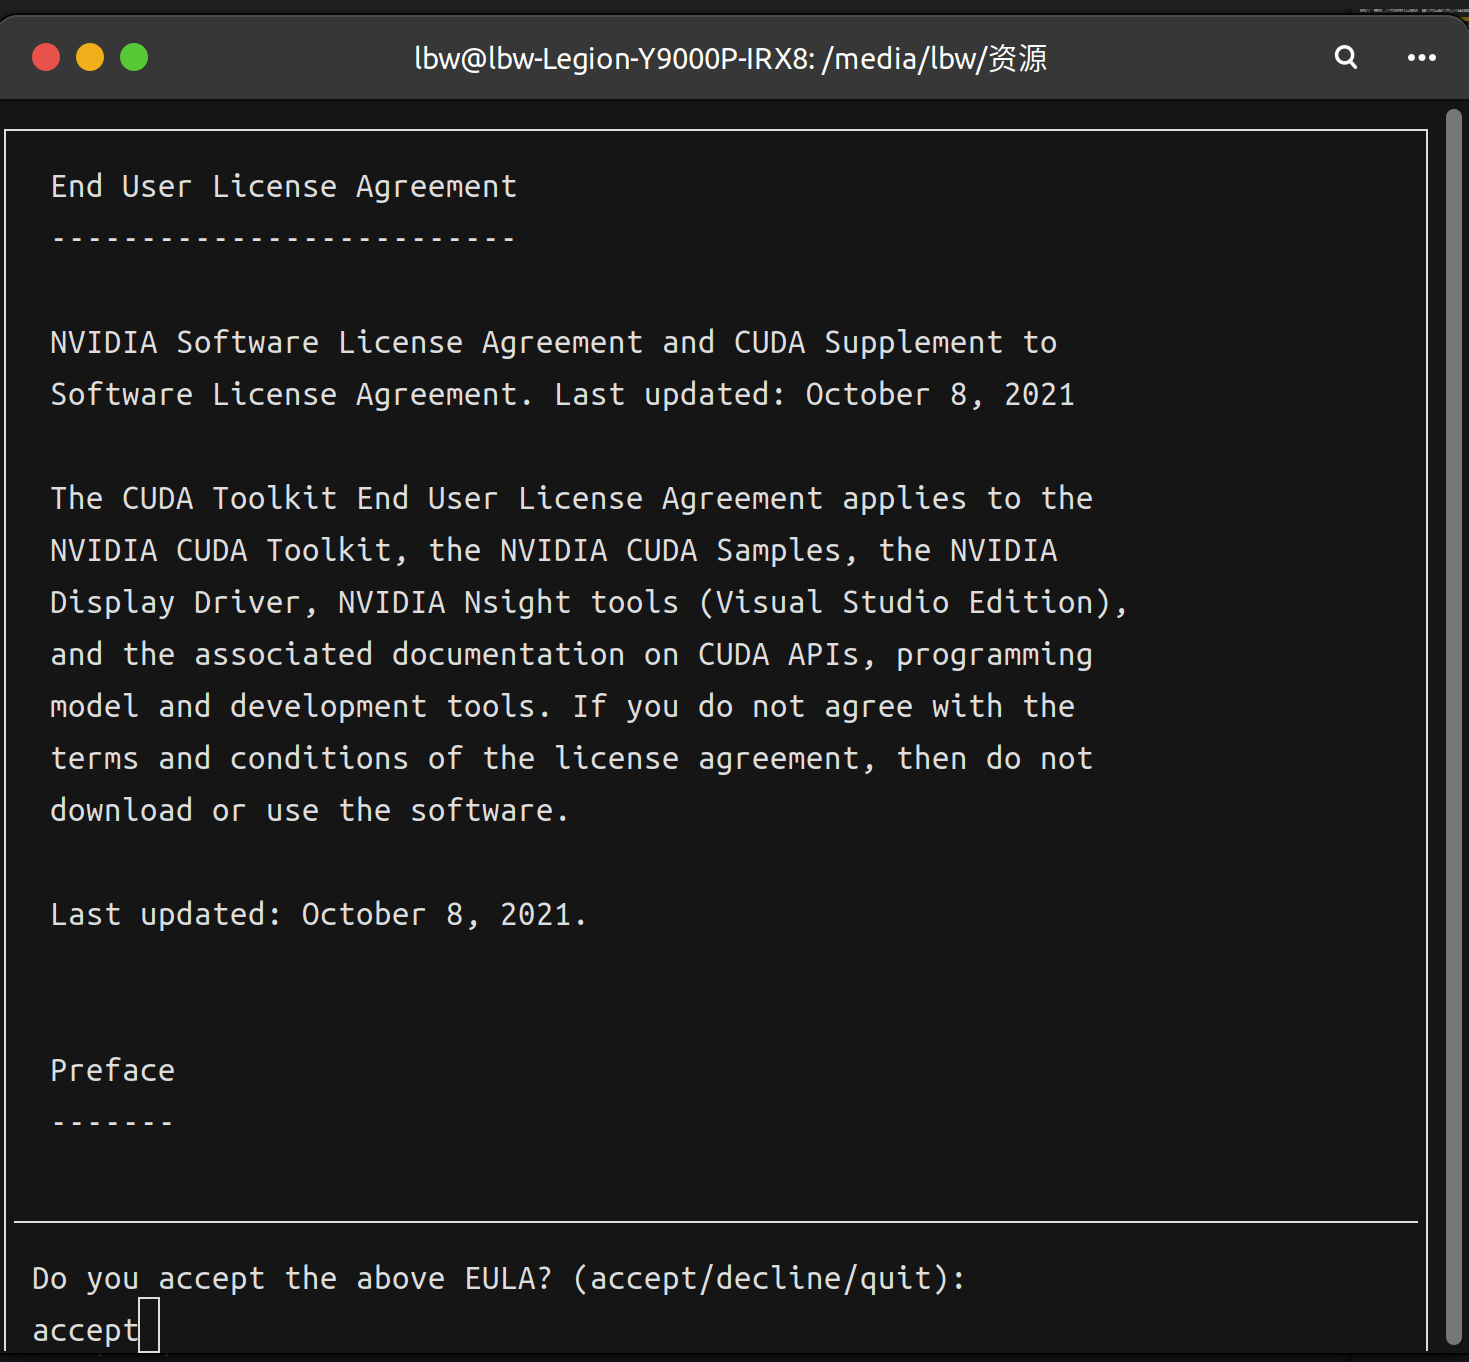
\includegraphics[width=0.7\textwidth]{CUDA_accept.png}
    \caption{Step2} % 图片标题
    \label{fig:CUDA_install} % 图片标签,用于引用
\end{figure}

输入\textbf{accept},进行下一步安装。

\begin{figure}[H]
    \centering
    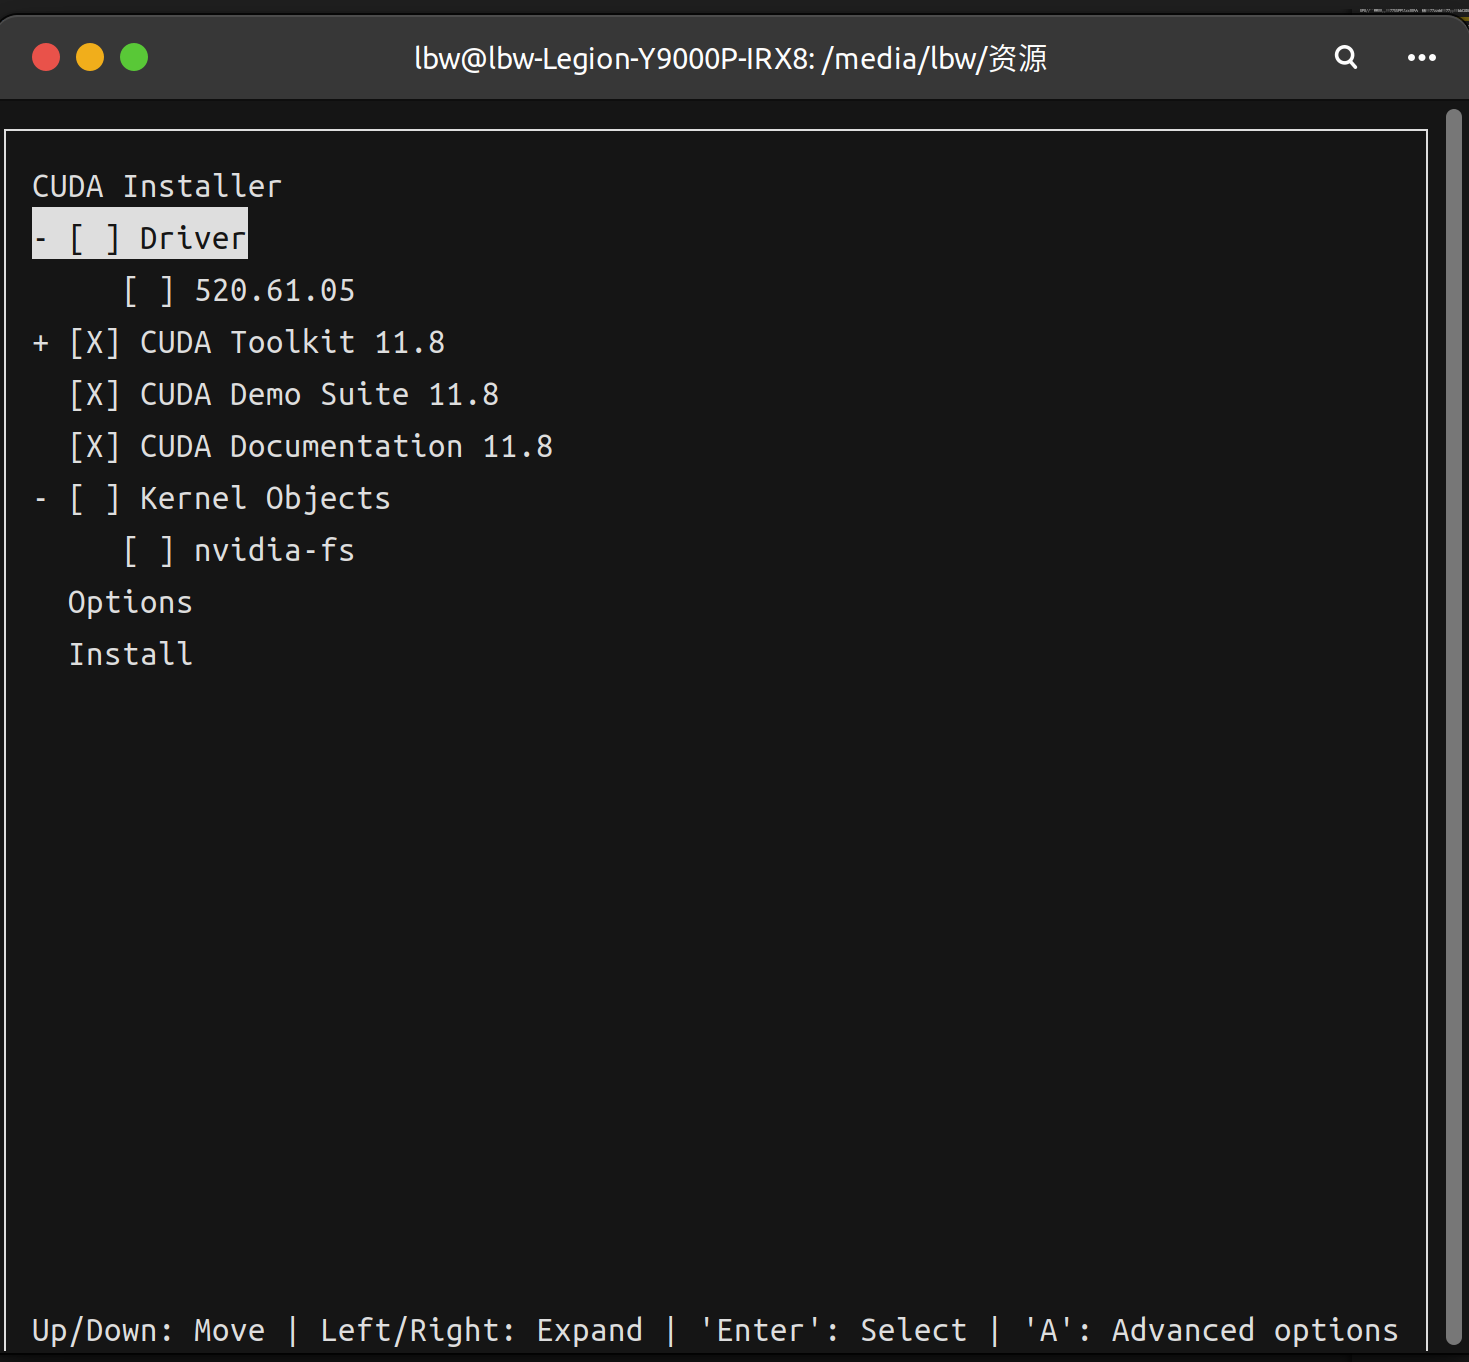
\includegraphics[width=0.7\textwidth]{CUDA_warning.png}
    \caption{Step3} % 图片标题
    \label{fig:CUDA_install} % 图片标签,用于引用
\end{figure}

这里需要特别注意,按下\textbf{Space}键,取消安装驱动,我们只安装toolkit。
\textbf{否则将会导致显卡掉驱动,严重者将导致屏幕无法亮起,请务必注意}。

完成后,请按照提示设置环境变量。然后就可以使用命令\textbf{nvcc}检测是否安装成功。

\begin{figure}[H]
    \centering
    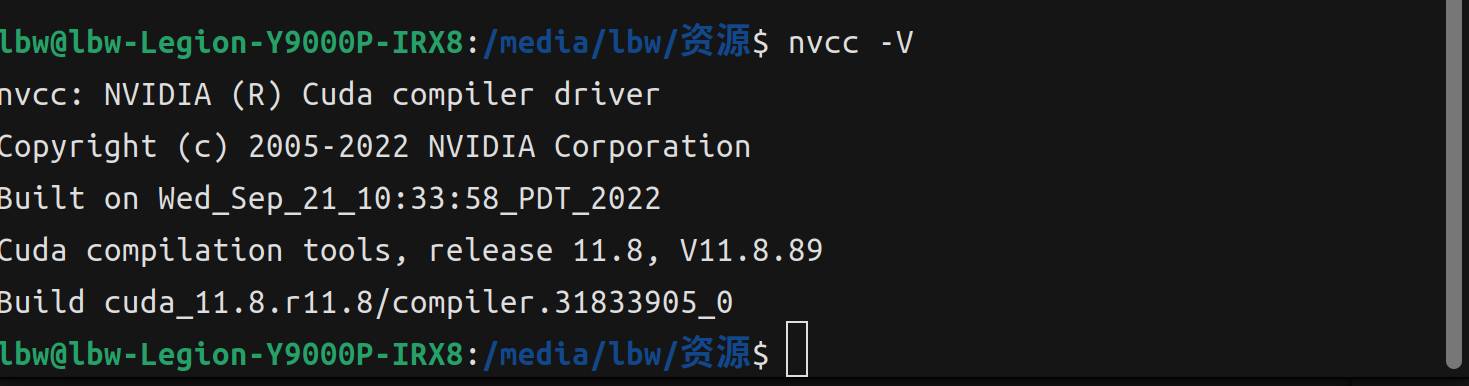
\includegraphics[width=0.7\textwidth]{CUDA_check.png}
    \caption{Step4} % 图片标题
    \label{fig:CUDA_install} % 图片标签,用于引用
\end{figure}

出现上图说明安装成功。

\subsubsection{安装cuDNN}

cuDNN是NVIDIA针对深度学习的深度神经网络加速库,可以加速卷积神经网络的运算。

推荐使用包解压的方式安装cuDNN,这样方便进行CUDA toolkit和cuDNN版本的管理。

\begin{tbash}
# 下载cuDNN安装包
wget https://developer.download.nvidia.com/compute/
redist/cudnn/v8.3.3/cudnn-11.8-linux-x64-v8.3.3.33.tgz

# 解压安装包
tar -xzvf cudnn-11.8-linux-x64-v8.3.3.33.tgz

# 移动cuDNN文件到CUDA安装目录
sudo cp cuda/include/cudnn*.h /usr/local/cuda/include
sudo cp cuda/lib64/libcudnn* /usr/local/cuda/lib64
sudo chmod a+r /usr/local/cuda/include/cudnn*.h /usr/local/cuda/lib64/libcudnn*
\end{tbash}

注意,只有在系统库中发现了cuDNN的库头文件和库文件,CUDA程序才可以正常使用。

\subsection{CUDA运行逻辑}

\subsubsection{异构计算架构}

GPU并不是一个独立运行的计算平台,而需要与CPU协同工作,可以看成是CPU的协处理器,CPU会对GPU进行任务下达和指令部署,因此当我们在说GPU并行计算时,其实是指的基于CPU+GPU的异构计算架构。

在异构计算架构中,GPU与CPU通过PCIe总线连接在一起来协同工作,CPU所在位置称为为主机端(host),而GPU所在位置称为设备端(device)

\begin{figure}[H]
    \centering
    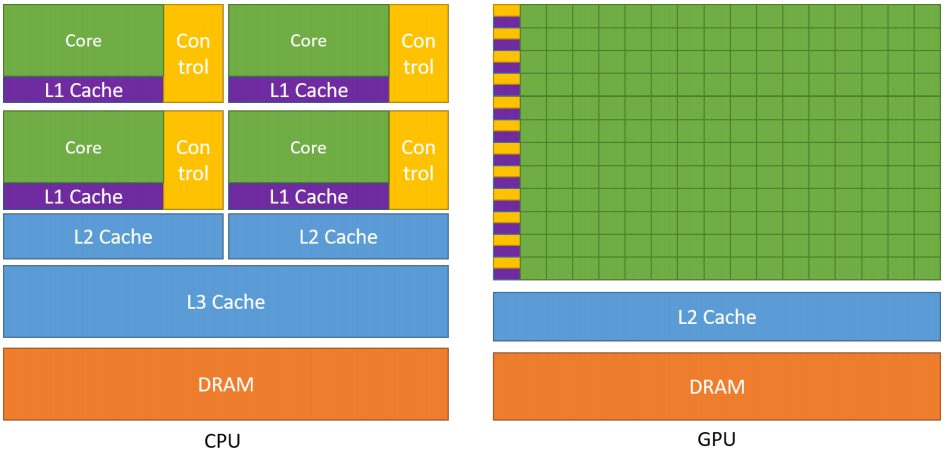
\includegraphics[width=0.85\textwidth]{Host-Device.png}
    \caption{CPU-GPU混合架构} % 图片标题
    \label{fig:CPU-GPU} % 图片标签,用于引用
\end{figure}

















\subsection{CUDA编程基础}
可以参考NVIDIA官方的CUDA编程指南\url{https://www.nvidia.cn/docs/IO/51635/NVIDIA_CUDA_Programming_Guide_1.1_chs.pdf}


